\documentclass[10pt, a4paper]{article} 
\usepackage[T1]{fontenc}
\usepackage{fontawesome} 
\usepackage[sfdefault]{roboto}
\usepackage[british]{babel}
\usepackage{ragged2e}
\usepackage[left=0mm, right=0mm, top=0mm, bottom=0mm]{geometry}
%\usepackage{microtype}
\usepackage[stretch=25, shrink=25, tracking=true, letterspace=30]{microtype}  
\usepackage{graphicx}        
\usepackage{xcolor}
\usepackage{pifont}
\usepackage{enumitem}
    
\setlist{parsep=0pt, topsep=0pt, partopsep=1pt, itemsep=1pt, leftmargin=6mm}       
\renewcommand{\familydefault}{\sfdefault}

\definecolor{cvblue}{HTML}{0F2666} %1E3A8A
\newcommand{\is}{\par\vskip.5ex plus .4ex} 

\newcommand{\job}[3]{%
    \is
    \textbf{\textsc{#1}}\\%
    \textbf{\textcolor{cvblue}{#2}} \dates{#3}
}

\newcommand{\education}[3]{%
    \is
    \textbf{\textsc{\textcolor{black}{#1}}}\\
    {#2}\\
    \dates{#3}
}

\newcommand{\cert}[3]{%
  #1 #2, \textit{#3}%
}

\newcommand{\dates}[1]{\hfill\mbox{#1}}
\newcommand{\headleft}[1]{\vspace*{3ex}\textsc{\textbf{#1}}\par%
    \vspace*{-1.5ex}\hrulefill\par\vspace*{0.7ex}}
\newcommand{\headright}[1]{\vspace*{2.5ex}\textsc{\Large\color{cvblue}#1}\par%
     \vspace*{-2ex}{\color{cvblue}\hrulefill}\par}

\usepackage[colorlinks = true, urlcolor = white, linkcolor = white]{hyperref}

\begin{document}

\setlength{\topskip}{0pt}
\setlength{\parindent}{0pt}
\setlength{\parskip}{0pt}
\setlength{\fboxsep}{0pt}
\pagestyle{empty}
\raggedbottom
\setlist[itemize]{leftmargin=1em, itemsep=0.5ex}

%%%%%%%%%%%%%%%%%%%%%%%%%%%%%%%%%%%%%%%%%%%%%%%%%%%%%%%
%                 LEFT COLUMN                      %
%%%%%%%%%%%%%%%%%%%%%%%%%%%%%%%%%%%%%%%%%%%%%%%%%%%%%%%
\begin{minipage}[t]{0.33\textwidth} 
\colorbox{cvblue}{\begin{minipage}[t][5mm][t]{\textwidth}\null\hfill\null\end{minipage}}

\vspace{-.2ex} 
\colorbox{cvblue!90}{\color{white}  
\kern0.09\textwidth\relax
\begin{minipage}[t][293mm][t]{0.82\textwidth}
\raggedright
\vspace*{2.5ex}

\Large Antonia \textbf{\textsc{Frey}} \normalsize 

\null\hfill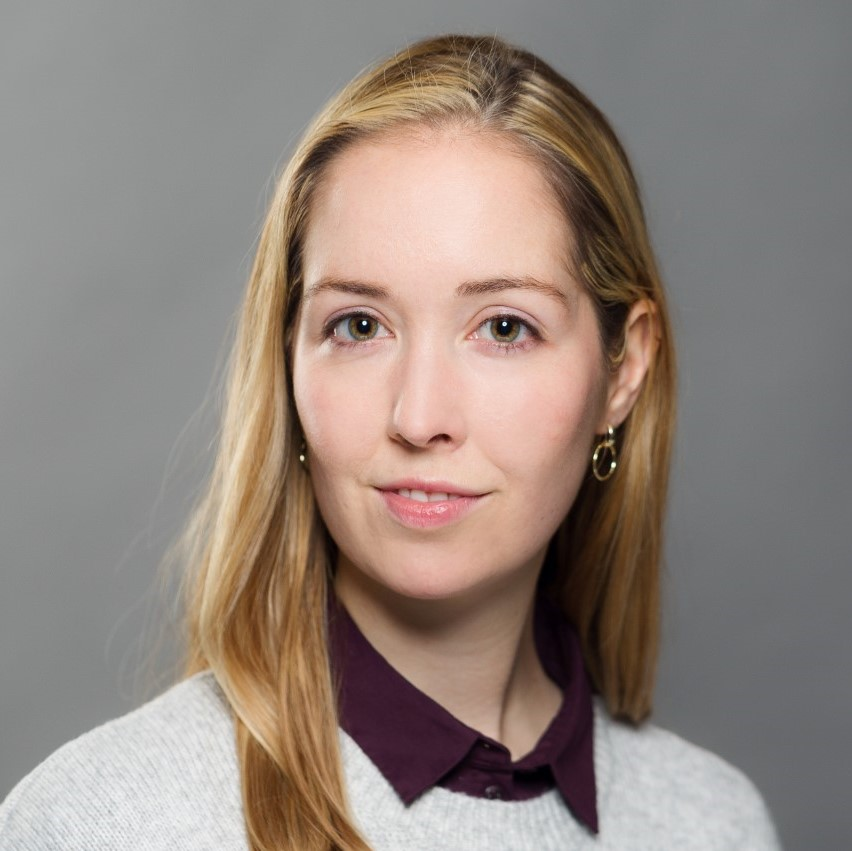
\includegraphics[width=0.65\textwidth]{aaf.jpg}\hfill\null

\vspace*{0.5ex} 

\headleft{Profile Summary}
\parbox{1\textwidth}{
{\small
\justifying
\noindent
Software Engineer with 4+ years of experience in Python, web development frameworks, and Java. Since the beginning of my career, I have contributed to diverse projects across industries like telecommunications, automotive, and energy, building applications from scratch, implementing new features, and solving complex problems in agile, international teams. As a team player, I thrive in collaborative environments, enjoying the opportunity to work together to achieve goals. Moreover, I value simplicity, thoughtful design, and creating maintainable solutions, with a strong emphasis on testing to ensure robust, reliable software. Beyond my technical skills, I am flexible, communicative, and always eager to learn new technologies and share knowledge.
}}


\headleft{Contact details}
{\small
\href{mailto:antonia.frey@outlook.com}{\faEnvelope\ antonia.frey@outlook.com} \\[0.4ex]
\href{https://wa.me/+4915146782868}{\faPhone\ +49 1514 6782868} \\[0.4ex]
\href{https://www.linkedin.com/in/antonia-alice-frey}{\faLinkedinSquare\ Antonia Alice Frey} \\[0.4ex]
\href{https://github.com/thebughuntress}{\faGithub\ thebughuntress} \\[0.4ex]
\href{https://antoniaalicefrey.com}{\faHome\ antoniaalicefrey.com} \\[0.4ex]
\faMapMarker\ Freiburg (DE) / Argentiere (FR)
}

\headleft{Personal information}
{\small
Citizenship: \textbf{Swiss, German} \\[0.5ex]
Languages:\\
\begin{itemize}[leftmargin=1em]
    \item \textbf{German} (C2)
        \item \textbf{English} (C1)
    \item \textbf{Spanish} (C1)
    \item \textbf{French} (B1)
\end{itemize}}

\headleft{Technologies \& Tools}
{\small
\begin{itemize}[leftmargin=1em]
    \item \textbf{Programming Languages}\\
    Python, TypeScript, Java
    \item \textbf{Frontend}\\
     React, Vue, Angular, Redux, Material UI, Bootstrap, Tailwind CSS, HTML/CSS
    \item \textbf{Backend}\\
    Python Django, NodeJS, MongoDB, SQL
    \item \textbf{Testing}\\
    Java/Selenium, Postman (API Testing), Cypress / Cucumber, Jest
    \item \textbf{Agile Practices}\\
     Git, CI/CD, SCRUM, Jira, Confluence
\end{itemize}
}

\end{minipage}%
\kern0.09\textwidth\relax
}
\end{minipage}
\hskip2.5em
\begin{minipage}[t]{0.56\textwidth}
\setlength{\parskip}{0.8ex}

\vspace{2ex}

%%%%%%%%%%%%%%%%%%%%%%%%%%%%%%%%%%%%%%%%%%%%%%%%%%%%%%%
%                 RIGHT COLUMN                      %
%%%%%%%%%%%%%%%%%%%%%%%%%%%%%%%%%%%%%%%%%%%%%%%%%%%%%%%

\headright{Experience}

\renewcommand{\labelitemi}{$\diamond$}

\job{Software Engineer · IT Consultant}
    {Devoteam GmbH, Frankfurt, Germany · Remote}
    {February 2022 -- Now}

\begin{itemize}
    \item Development of web applications, leveraging cloud technologies, for data visualization using modern frameworks like React, Vue, and TypeScript/JavaScript.
 \item Translating client requirements into technical solutions, participating in meetings to ensure alignment with stakeholder expectations, and delivering urgent fixes
    \item Implemented Git integration within GitLab CI/CD pipelines to optimize version control and automate deployment workflows.
    \item Test automation with Java/Selenium, Cypress, and unit testing with Jest
    \item Collaborated in an Agile Scrum environment using Git, Jira, and Confluence to manage tasks and document workflows.
\end{itemize}

\job{Junior Python Programmer · System Analyst}
    {ELCA Informatique SA, Granada, Spain · Switzerland}  
    {Jan. 2021 -- Jan. 2022}

\begin{itemize}
    \item Automation of business-critical processes and implementation of new functionality in the company-wide production ERP system with Python.
    \item Programming and changing VBA scripts to generate business reports.
    \item Querying databases using SQL to ensure data accuracy and integrity.
    \item Performing business analysis for new features, drafting user stories and acceptance criteria, and coordinating client meetings with stakeholders in Switzerland while collaborating within an international team comprising Spanish, German, and French-speaking colleagues.
\end{itemize}

\job{Software Engineer (Internship)}
    {Intel Labs, Karlsruhe, Germany}  
    {Aug. 2019 -- Jan. 2020}

\begin{itemize}
    \item Automotive software development for an open-source simulator (CARLA.org) for autonomous driving research.
    \item Creating traffic scenarios which describe traffic situations and vehicle behaviors like a lane change (with Python).
    \item Debugging, testing, and implementing unsupported Parser features.
\end{itemize}

\job{System Engineer (Internship)}
    {BMW M, Munich, Germany}  
    {Sep. 2018 -- Feb. 2019}
    
\begin{itemize}
    \item Developing a Windows desktop app with C\# to automatically translate bus communication protocols from LIN to CAN and vice versa.
    \item Antenna measurements during test drives in disguised prototype cars.
    \item Organization of the annual tire change for vehicle fleets in coordination with vehicle bookings and mechanics as well as measurement and technical documentation of wheelbase parameters.
\end{itemize}


%%%%%%%%%% EDUCATION %%%%%%%%%%

\headright{Education}

\education{M. Sc. Electrical Engineering and Information Technology}
          {Karlsruhe Institute of Technology (KIT)}
          {2018 -- 2020}

\education{B. Sc. Electrical Engineering and Information Technology}
          {Karlsruhe Institute of Technology (KIT)}
          {2013 -- 2018}


%%%%%%%%%% CERTIFICATIONS %%%%%%%%%%
\headright{Certifications}

\begin{itemize}
\item \cert{2025}{ISTQB Certified Tester Foundation Level}{atsqa.org}
\item \cert{2024}{Professional Python Programmer Level 1}{pythoninstitute.org}
\item \cert{2023}{AWS Certified Cloud Practitioner}{Amazon}
\item \cert{2023}{Google Cloud Engineer}{Google}
\item \cert{2023}{Google Cloud Digital Leader}{Google}
\item \cert{2022}{Professional Scrum Master I}{scrum.org}
\end{itemize}



\end{minipage}

\end{document}
